\begin{pastexam}[label={px:ccu-108-swa-02}]{中正資工所甲組 108 學年度 第 3 題}
（追蹤）

(6\%) To build a max heap, the following key values are inserted in the given order: 7, 16, 49,
82, 5, 31, 6, 2, 44.
\begin{enumerate}[label=(\alph*)]
\item (3\%) Please write down the status of the max heap after \textbf{all} values are inserted
into the max heap.
\item (3\%) Starting with the max heap built in (a), please write down the status of the max heap
as well as the sorted array after the \textbf{5-th} iteration during the heap sort. Note that each
iteration swaps the first and the last records in the current heap, and then rearranges records
so that the record with maximum key is moved to its correct position in the sorted array and the
remaining heap is still a max heap.
\end{enumerate}
\end{pastexam}

\begin{pastsoln}
答案：(a) 用陣列寫是 $\langle 82, 49, 31, 44, 5, 16, 6, 2, 7\rangle$；(b) 第 $5$ 回合結束時，整個陣列是
$\langle 7, 5, 6, 2 \mid 16, 31, 44, 49, 82\rangle$，前四格是堆積，後五格是排好的部分。

堆積用陣列 $A[1..9]$ 存，$A[i]$ 的父節點是 $A[\lfloor i/2 \rfloor]$，子節點是 $A[2i]$、
$A[2i+1]$（資結書第~8.1~節）。

\textbf{(a)} 題目說「依序插入」，所以每個數放到最後一格，再往上浮（和父節點比，比父節點大就交換）。
這和一次拿到全部的數再由下而上建堆積（資結書第~8.2~節）是不同的做法，結果也可能不同。

\begin{center}
\begin{tabular}{cll}
\toprule
插入 & 上浮的過程 & 插入後的陣列 \\
\midrule
7 & 第一個數，放在 $A[1]$ & $7$ \\
16 & $A[2] = 16 > A[1] = 7$，交換 & $16, 7$ \\
49 & $A[3] = 49 > A[1] = 16$，交換 & $49, 7, 16$ \\
82 & $A[4]$：$82 > 7$ 和 $A[2]$ 交換；$82 > 49$ 和 $A[1]$ 交換 & $82, 49, 16, 7$ \\
5 & $A[5]$：$5 < 49$，不動 & $82, 49, 16, 7, 5$ \\
31 & $A[6]$：$31 > 16$ 和 $A[3]$ 交換；$31 < 82$ 停 & $82, 49, 31, 7, 5, 16$ \\
6 & $A[7]$：$6 < 31$，不動 & $82, 49, 31, 7, 5, 16, 6$ \\
2 & $A[8]$：$2 < 7$，不動 & $82, 49, 31, 7, 5, 16, 6, 2$ \\
44 & $A[9]$：$44 > 7$ 和 $A[4]$ 交換；$44 < 49$ 停 & $82, 49, 31, 44, 5, 16, 6, 2, 7$ \\
\bottomrule
\end{tabular}
\end{center}

全部插入後的最大堆積：

\begin{center}
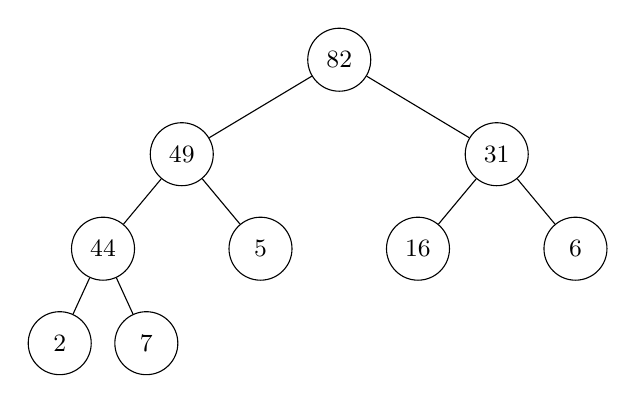
\begin{tikzpicture}[
    every node/.style={circle, draw, minimum size=8mm, inner sep=0pt, font=\small},
    level distance=12mm,
    level 1/.style={sibling distance=40mm},
    level 2/.style={sibling distance=20mm}, level 3/.style={sibling distance=11mm}]
\node {82}
  child {node {49}
    child {node {44} child {node {2}} child {node {7}}}
    child {node {5}}}
  child {node {31}
    child {node {16}}
    child {node {6}}};
\end{tikzpicture}
\end{center}

\textbf{(b)} 堆積排序（資結書第~14.6~節）每一回合把 $A[1]$（目前最大）和堆積的最後一格交換，
堆積大小減 $1$，再讓新的 $A[1]$ 往下沉（和較大的子節點比，比它小就交換）。 下表的「$\mid$」
右邊是已經排好的部分。

\begin{center}
\small
\begin{tabular}{cll}
\toprule
回合 & 交換與下沉 & 回合結束時的陣列 \\
\midrule
1 & $82 \leftrightarrow 7$；$7$ 和 $49$ 換，再和 $44$ 換 & $49, 44, 31, 7, 5, 16, 6, 2 \mid 82$ \\
2 & $49 \leftrightarrow 2$；$2$ 和 $44$ 換，再和 $7$ 換 & $44, 7, 31, 2, 5, 16, 6 \mid 49, 82$ \\
3 & $44 \leftrightarrow 6$；$6$ 和 $31$ 換，再和 $16$ 換 & $31, 7, 16, 2, 5, 6 \mid 44, 49, 82$ \\
4 & $31 \leftrightarrow 6$；$6$ 和 $16$ 換，$A[3]$ 沒有子節點了 & $16, 7, 6, 2, 5 \mid 31, 44, 49, 82$ \\
5 & $16 \leftrightarrow 5$；$5$ 和 $7$ 換，$5 > A[4] = 2$ 停 & $7, 5, 6, 2 \mid 16, 31, 44, 49, 82$ \\
\bottomrule
\end{tabular}
\end{center}

逐回合說明下沉時比的是哪兩個子節點：
\begin{itemize}
\item 第 $1$ 回合：堆積剩 $A[1..8]$。 $7$ 的子節點 $49, 31$，和 $49$ 換到 $A[2]$；子節點
$44, 5$，和 $44$ 換到 $A[4]$；子節點只剩 $A[8] = 2 < 7$，停。
\item 第 $2$ 回合：堆積剩 $A[1..7]$。 $2$ 的子節點 $44, 31$，換到 $A[2]$；子節點 $7, 5$，換到
$A[4]$；$A[8]$ 已不在堆積裡，停。
\item 第 $3$ 回合：堆積剩 $A[1..6]$。 $6$ 的子節點 $7, 31$，換到 $A[3]$；子節點只有 $A[6] = 16$，
$16 > 6$，換到 $A[6]$。
\item 第 $4$ 回合：堆積剩 $A[1..5]$。 $6$ 的子節點 $7, 16$，換到 $A[3]$；$A[6]$ 已不在堆積裡，停。
\item 第 $5$ 回合：堆積剩 $A[1..4]$。 $5$ 的子節點 $7, 6$，換到 $A[2]$；子節點 $A[4] = 2 < 5$，停。
\end{itemize}

第 $5$ 回合結束時，最大堆積是 $\langle 7, 5, 6, 2\rangle$（$7$ 是根，$5$、$6$ 是它的兩個子節點，
$2$ 是 $5$ 的左子節點），排好的部分是 $\langle 16, 31, 44, 49, 82\rangle$，整個陣列
$\langle 7, 5, 6, 2, 16, 31, 44, 49, 82\rangle$。
\end{pastsoln}
